\documentclass[openany]{book}

\usepackage[margin=1in]{geometry}
\usepackage{amsmath,amsfonts,amsthm, amssymb}
\usepackage{yhmath}
\usepackage{mathrsfs}
\usepackage{mathtools}
\usepackage{xcolor}
\usepackage{graphicx}
\usepackage{comment}
\usepackage{tikz-cd}
\usepackage{quiver}
\renewcommand{\familydefault}{ppl}
\newcommand{\tr}{\text{tr}}
\newcommand{\R}{\mathbb{R}}
\newcommand{\E}{\mathbb{E}}
\newcommand{\Z}{\mathbb{Z}}
\newcommand{\C}{\mathbb{C}}
\newcommand{\F}{\mathbb{F}}
\newcommand{\la}{\langle}
\newcommand{\ra}{\rangle}
\newcommand{\colim}{\text{colim}}
\DeclareMathOperator{\im}{im}
\let\oldemptyset\emptyset
\let\emptyset\varnothing
\newcommand{\tor}{\text{Tor}}
\newcommand{\id}{\text{id}}
\newcommand{\ext}{\text{Ext}}
\newcommand{\ptop}{\text{PTop}}
\newcommand{\pt}{\text{pt}}
\newcommand{\ach}{\text{Ach}}
\newcommand{\Q}{\mathbb{Q}}
\newcommand{\gal}{\text{Gal}}


\usepackage{thmtools,thm-restate}

% Fixing mdframed skip below
% See https://tex.stackexchange.com/a/292090/143086
\usepackage[framemethod=TikZ]{mdframed}
\usepackage{xpatch}
\makeatletter
\xpatchcmd{\endmdframed}
	{\aftergroup\endmdf@trivlist\color@endgroup}
	{\endmdf@trivlist\color@endgroup\@doendpe}
	{}{}
\makeatother

\definecolor{huilightpink}{HTML}{fff2fe}
\definecolor{huidarkpink}{HTML}{d955b7}
\declaretheoremstyle[
	mdframed={
		backgroundcolor=huilightpink,
		linecolor=huidarkpink,
		rightline=false,
		topline=false,
		bottomline=false,
		linewidth=2pt,
		innertopmargin=5pt,
		innerbottommargin=8pt,
		innerleftmargin=8pt,
		leftmargin=-2pt,
		skipbelow=2pt,
		nobreak
	},
	headfont=\normalfont\bfseries\color{huidarkpink}
]{huipinkbox}
\declaretheorem[style=huipinkbox,name=Theorem,within=chapter]{thm}
\declaretheorem[style=huipinkbox,name=Theorem,sibling=thm]{theorem}




\begin{comment}
\definecolor{huilightyellow}{HTML}{fff5d6}
\definecolor{huidarkyellow}{HTML}{fcad03}
\declaretheoremstyle[
	mdframed={
		backgroundcolor=huilightyellow,
		linecolor=huidarkyellow,
		rightline=false,
		topline=false,
		bottomline=false,
		linewidth=2pt,
		innertopmargin=5pt,
		innerbottommargin=8pt,
		innerleftmargin=8pt,
		leftmargin=-2pt,
		skipbelow=2pt,
		nobreak
	},
	headfont=\normalfont\bfseries\color{huidarkyellow}
]{huiyellowbox}
\declaretheorem[style=huiyellowbox,name=Proposition,within=chapter]{prop}
\end{comment}



\definecolor{huilightpurple}{HTML}{faf2ff}
\definecolor{huidarkpurple}{HTML}{912ed9}
\declaretheoremstyle[
	mdframed={
		backgroundcolor=huilightpurple,
		linecolor=huidarkpurple,
		rightline=false,
		topline=false,
		bottomline=false,
		linewidth=2pt,
		innertopmargin=5pt,
		innerbottommargin=8pt,
		innerleftmargin=8pt,
		leftmargin=-2pt,
		skipbelow=2pt,
		nobreak
	},
	headfont=\normalfont\bfseries\color{huidarkpurple}
]{huipurplebox}
\declaretheorem[style=huipurplebox,name=Proposition,within=chapter]{prop}



% \definecolor{huilightpurple}{HTML}{faf2ff}
% \definecolor{huidarkpurple}{HTML}{912ed9}
% \declaretheoremstyle[
% 	mdframed={
% 		backgroundcolor=huilightpurple,
% 		linecolor=huidarkpurple,
% 		rightline=false,
% 		topline=false,
% 		bottomline=false,
% 		linewidth=2pt,
% 		innertopmargin=5pt,
% 		innerbottommargin=8pt,
% 		innerleftmargin=8pt,
% 		leftmargin=-2pt,
% 		skipbelow=2pt,
% 		nobreak
% 	},
% 	headfont=\normalfont\bfseries\color{huidarkpurple}
% ]{huipurplebox}
\declaretheorem[style=huipurplebox,name=Lemma,within=chapter]{lem}


\definecolor{lightpink}{HTML}{f0f6fc}
\definecolor{darkpink}{HTML}{2c72b8}
\declaretheoremstyle[
	mdframed={
		backgroundcolor=lightpink,
		linecolor=darkpink,
		rightline=false,
		topline=false,
		bottomline=false,
		linewidth=2pt,
		innertopmargin=5pt,
		innerbottommargin=8pt,
		innerleftmargin=8pt,
		leftmargin=-2pt,
		skipbelow=2pt,
		nobreak
	},
	headfont=\normalfont\bfseries\color{darkpink}
]{pinkbox}
\declaretheorem[style=pinkbox,name=Definition,within=chapter]{defn}


\definecolor{huilightblue}{HTML}{edf9ff}
\definecolor{huidarkblue}{HTML}{4b79db}
\declaretheoremstyle[
	mdframed={
		backgroundcolor=huilightblue,
		linecolor=huidarkblue,
		rightline=false,
		topline=false,
		bottomline=false,
		linewidth=2pt,
		innertopmargin=5pt,
		innerbottommargin=8pt,
		innerleftmargin=8pt,
		leftmargin=-2pt,
		skipbelow=2pt,
		nobreak
	},
	headfont=\normalfont\bfseries\color{huidarkblue}
]{huiblueblox}
\declaretheorem[style=huiblueblox,name=Example,within=chapter]{example}



% \definecolor{huilightblue}{HTML}{edf9ff}
% \definecolor{huidarkblue}{HTML}{4b79db}
% \declaretheoremstyle[
% 	mdframed={
% 		backgroundcolor=huilightblue,
% 		linecolor=huidarkblue,
% 		rightline=false,
% 		topline=false,
% 		bottomline=false,
% 		linewidth=2pt,
% 		innertopmargin=5pt,
% 		innerbottommargin=8pt,
% 		innerleftmargin=8pt,
% 		leftmargin=-2pt,
% 		skipbelow=2pt,
% 		nobreak
% 	},
% 	headfont=\normalfont\bfseries\color{huidarkblue}
% ]{huiblueblox}
% \declaretheorem[style=huiblueblox,name=Example,within=chapter]{example}

% \declaretheoremstyle[
% 	mdframed={
% 		backgroundcolor=huilightblue,
% 		linecolor=huidarkblue,
% 		rightline=false,
% 		topline=false,
% 		bottomline=false,
% 		linewidth=2pt,
% 		innertopmargin=5pt,
% 		innerbottommargin=8pt,
% 		innerleftmargin=8pt,
% 		leftmargin=-2pt,
% 		skipbelow=2pt,
% 		nobreak
% 	},
% 	headfont=\normalfont\bfseries\color{huidarkblue}
% ]{huiblueblox}
\declaretheorem[style=huiblueblox,name=Problem,within=chapter]{prob}



% \declaretheoremstyle[
% 	mdframed={
% 		backgroundcolor=huilightblue,
% 		linecolor=huidarkblue,
% 		rightline=false,
% 		topline=false,
% 		bottomline=false,
% 		linewidth=2pt,
% 		innertopmargin=5pt,
% 		innerbottommargin=8pt,
% 		innerleftmargin=8pt,
% 		leftmargin=-2pt,
% 		skipbelow=2pt,
% 		nobreak
% 	},
% 	headfont=\normalfont\bfseries\color{huidarkblue}
% ]{huiblueblox}
\declaretheorem[style=huiblueblox,name=Exercise,within=chapter]{exer}
\declaretheorem[style=huipinkbox, name=Corollary, within=chapter]{cor}





















\newcommand{\nirwarnsymbol}{%
	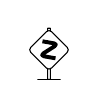
\begin{tikzpicture}[baseline=(x.base)]
		\draw[rounded corners=.01em] (-.05em,-1.07em)rectangle(.05em,.78em);
		\draw[fill=white,rounded corners=1.3] (0,.75em)--(.75em,0)--(0,-.75em)--(-.75em,0)--cycle;
		\draw[line width=0.2mm, line cap=round](-.4em,-1.07em)--(.4em,-1.07em);
		\node(x) at (0,0em) {};
		% Thank you https://tex.stackexchange.com/a/262510
		\draw[
			line cap=but,
			line join=round,
			x=.5em,
			line width=0.5mm,
			y=1*(height("Z")-\pgflinewidth)*(1-sin(10)),
			rotate=-10,
			rounded corners=1.5pt,
		](-0.57, 0.57) -- (0.57, 0.57) -- (-0.57, -0.57) -- (0.57, -0.57);
	\end{tikzpicture}%
}

%%%%%%%%%%%%%%%%%%%%%%%%%%%%%%%%%%%%%%%%%%%% MARGINS
\usepackage{marginnote}
% Thank you https://tex.stackexchange.com/a/472882
% Makes marginnotes always appear on the left, apparently
%
\makeatletter
\long\def\@mn@@@marginnote[#1]#2[#3]{%
	\begingroup
		\ifmmode\mn@strut\let\@tempa\mn@vadjust\else
			\if@inlabel\leavevmode\fi
			\ifhmode\mn@strut\let\@tempa\mn@vadjust\else\let\@tempa\mn@vlap\fi
		\fi
		\@tempa{%
			\vbox to\z@{%
				\vss
				\@mn@margintest
				\if@reversemargin\if@tempswa
						\@tempswafalse
					\else
						\@tempswatrue
				\fi\fi

					\llap{%
						\vbox to\z@{\kern\marginnotevadjust\kern #3
							\vbox to\z@{%
								\hsize\marginparwidth
								\linewidth\hsize
								\kern-\parskip
								%\mn@parboxrestore
								\marginfont\raggedleftmarginnote\strut\hspace{\z@}%
								\ignorespaces#1\endgraf
								\vss
							}%
							\vss
						}%
						\if@mn@verbose
							\PackageInfo{marginnote}{xpos seems to be \@mn@currxpos}%
						\fi
						\begingroup
							\ifx\@mn@currxpos\relax\else\ifx\@mn@currpos\@empty\else
									\kern\@mn@currxpos
							\fi\fi
							\ifx\@mn@currpage\relax
								\let\@mn@currpage\@ne
							\fi
							\if@twoside\ifodd\@mn@currpage\relax
									\kern-\oddsidemargin
								\else
									\kern-\evensidemargin
								\fi
							\else
								\kern-\oddsidemargin
							\fi
							\kern-1in
						\endgroup
						\kern\marginparsep
					}%
			}%
		}%
	\endgroup
}
\makeatother
%
% Mostly for todonotes
\renewcommand{\marginpar}{\marginnote}
%%%%%%%%%%%%%%%%%%%%%%%%%%%%%%%%%%%%%%%%%%%% /MARGINS

\definecolor{nirlightred}{RGB}{250, 220, 220}
\definecolor{nirdarkred}{HTML}{f40000}
\declaretheoremstyle[
	mdframed={
		backgroundcolor=nirlightred,
		linecolor=nirdarkred,
		rightline=false,
		topline=false,
		bottomline=false,
		linewidth=2pt,
		innertopmargin=5pt,
		innerbottommargin=8pt,
		innerleftmargin=8pt,
		leftmargin=-2pt,
		skipbelow=2pt,
		nobreak
	},
	headfont=\normalfont\bfseries\color{nirdarkred}
]{nirredbox}

% \makeatletter
% \declaretheorem[
% 	style=nirredbox,
% 	name=Warning,
% 	sibling=thm,
% 	% without \leavevmode, the first item in a list gets misformatted
% 	postheadhook={\leavevmode\marginnote{\nirwarnsymbol}[-3pt]%
% 	\ifthmt@thisistheone% restatable makes alignment weird
% 		\hspace{-2.2pt}%
% 	\fi}
% ]{warn}
% \makeatother

\newcommand{\nirideasymbol}{%
	
\begin{tikzpicture}[baseline=(x.base)]
		\draw[rounded corners=.01em] (-.05em,-1.07em)rectangle(.05em,.78em);
		\draw[fill=white,rounded corners=1.3] (0,.75em)--(.75em,0)--(0,-.75em)--(-.75em,0)--cycle;
		\draw[line width=0.2mm, line cap=round](-.4em,-1.07em)--(.4em,-1.07em);
		\node(x) at (0,0em) {};
		\node at (0,0em) {{\textbf{!}}};
	\end{tikzpicture}%
}
\renewcommand{\nirwarnsymbol}{%
	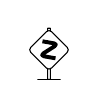
\begin{tikzpicture}[baseline=(x.base)]
		\draw[rounded corners=.01em] (-.05em,-1.07em)rectangle(.05em,.78em);
		\draw[fill=white,rounded corners=1.3] (0,.75em)--(.75em,0)--(0,-.75em)--(-.75em,0)--cycle;
		\draw[line width=0.2mm, line cap=round](-.4em,-1.07em)--(.4em,-1.07em);
		\node(x) at (0,0em) {};
		% Thank you https://tex.stackexchange.com/a/262510
		\draw[
			line cap=but,
			line join=round,
			x=.5em,
			line width=0.5mm,
			y=1*(height("Z")-\pgflinewidth)*(1-sin(10)),
			rotate=-10,
			rounded corners=1.5pt,
		](-0.57, 0.57) -- (0.57, 0.57) -- (-0.57, -0.57) -- (0.57, -0.57);
	\end{tikzpicture}%
}
\makeatletter
\declaretheorem[
	style=nirredbox,
	name=Idea,
	sibling=thm,
	% without \leavevmode, the first item in a list gets misformatted
	postheadhook={\leavevmode\marginnote{\nirideasymbol}[-3pt]%
	\ifthmt@thisistheone% restatable makes alignment weird
		\hspace{-2.2pt}%
	\fi}
]{idea}

\declaretheorem[
	style=nirredbox,
	name=Warning,
	sibling=thm,
	% without \leavevmode, the first item in a list gets misformatted
	postheadhook={\leavevmode\marginnote{\nirwarnsymbol}[-3pt]%
	\ifthmt@thisistheone% restatable makes alignment weird
		\hspace{-2.2pt}%
	\fi}
]{warn}
\makeatother

\title{Calc III Sections
\\ 
\vspace{0.4cm}
\large Fall 2025}




\date{\today}
\author{Hui Sun}


\begin{document}

\maketitle

% \tableofcontents
\newpage


\begin{center}
    \Large Calc III-Week 4 (9/15-9/19)
\end{center}

\renewcommand\thesection{\arabic{section}}

\noindent
Topics: (1) Partial derivatives. (2) 

\begin{defn}[graph]
    The \textbf{image} of a function $f: \R^n\to\R^m$ is a subset of $\R^m$,
    \begin{equation*}
        \text{Image}(f)=\{f(x)\in\R^m: x\in\R^n\}
    \end{equation*}
    and the \textbf{graph} of $f$ is a subset of $\R^{n+m}$,
    \begin{equation*}
        \text{Graph}(f)=\{(x,f(x)): x\in\R^n\}
    \end{equation*}
\end{defn}



\begin{defn}[limit]
    Let $f: A\subset\R^n\to\R^m$, ($A$ is open), let $N$ be a neighborhood of a point $b\in\R^m$. Now let $x$ approach $x_0$ ($x_0\in\bar{A}$,) $f$ is said to be \textbf{eventually in $N$} if there exists a neighborhood $U$ of $x_0$ such that whenever $x\in U$, then $f(x)\in N$ as well. 

    The \textbf{limit} of $f$ as $x\to x_0$, if it exists, is $\lim_{x\to x_0}f(x):=b\in\R^m$ such that $f$ is eventually in $N$, for every neighborhood $N$ of $b$. 
\end{defn}

\begin{defn}[limit']
    $\lim_{x\to x'}f(x)=b$ is when $x=(x_1, x_2, \dots, x_n)\to x'=(x_1',x_2',\dots, x_n')$ from \textbf{all directions}, $f(x)$ approaches $b=(b_1,\dots, b_m)$.
\end{defn}



\begin{defn}[continuity]
    Let $f:A\subset\R^n\to\R^m$ is said to be \textbf{continuous} at $x_0\in A$ if 
    \begin{equation*}
        \lim_{x\to x_0}f(x)=f(x_0)
    \end{equation*}
    And $f$ is called continuous if $f$ is continuous at every $x_0\in A$.
\end{defn}

\begin{example}
    The limit doesn't need to exist! For example, let 
    \begin{equation*}
        H(x)=\begin{cases}
            1, x\geq 0\\
            -1, x<0
        \end{cases}
    \end{equation*}
    Note the limit doesn't exist at $x=0$.
\end{example}




\begin{prob}
    For the following functions, find their (1) image, (2) graph, (3) draw their graphs.
    \begin{enumerate}
        \item  Let $f: \R\to\R$, and $f(x)=x^2+1$.
        \item Let $g: \R^2\to \R$, and $g(x)=x^2+y^2$.
    \end{enumerate}
\end{prob}


\begin{prob}
    Compute the following limits:
    \begin{enumerate}
        \item \begin{equation*}
            \lim_{(x,y)\to (0,0)}\frac{\sin xy}{y}
        \end{equation*}
       ( Hint: try writing $\frac{\sin xy}{y}=\frac{\sin xy}{xy}\cdot x$, and recall $\lim_{t\to 0}\frac{\sin t}{t}=1$).
        \item \begin{equation*}
            \lim_{(x,y)\to(0,0)}\frac{e^{xy}-1}{y}
        \end{equation*}
        \item \begin{equation*}
            \lim_{(x,y)\to(0,0)}\frac{(x-y)^2}{x^2+y^2}
        \end{equation*}
    \end{enumerate}
\end{prob}
\begin{proof}
    \begin{enumerate}
        \item Following the hint, we see 
        \begin{equation*}
            \lim_{(x,y)\to(0,0)}\frac{\sin xy}{y}=\lim_{(x,y)\to(0,0)}\frac{\sin xy}{xy}x=\lim_{x\to 0}x=0
        \end{equation*}
        \item This one uses the exact same trick: \begin{equation*}
            \lim_{(x,y)\to(0,0)}\frac{e^{xy}-1}{xy}\cdot y=0
        \end{equation*}
        \item First letting $x\to 0$ along $y=0$, we see the limit is $1$; letting $x=y\to 0$, we see the limit is $0$, thus the limit doesn't exist!
    \end{enumerate}
\end{proof}


\begin{prob}
    Compute the limit of the following functions:
    \begin{enumerate}
        \item \begin{equation*}
            \lim_{(x,y)\to(0,0)}\frac{x}{x+y} 
        \end{equation*}
        \item \begin{equation*}
            \lim_{(x,y)\to(0,0)}\frac{xy}{x+y}
        \end{equation*}
        (Hint: try considering $y=x^2-x$ and $y=x$)
        \item \begin{equation*}
            \lim_{(x,y)\to (0,0)}\frac{\sin(xy)}{x+y}
        \end{equation*}
        % \item $f(x,y)=\frac{x}{x+y}$ as $(x,y)\to (0,0)$.
        % \item $g(x,y)=\frac{xy}{x+y}$ as $(x,y)\to (0,0)$.
        % \item $h(x,y)=\frac{\sin(xy)}{x+y}$ as $(x,y)\to (0,0)$. Recall that $\lim_{x\to 0}\frac{\sin(x)}{x}=1$.
    \end{enumerate}
\end{prob}
\begin{proof}
    \begin{enumerate}
        \item First fix $x=0$, let $y\to 0$, then the limit is $0$; now fix $y=0$, let $x\to 0$, the limit is $1$. The limit doesn't exist!
        \item 
      %
        % \begin{equation*}
        %     \lim_{(x,y)\to(0,0)}\frac{xy}{x+y}=\lim_{(x,y)}\frac{x}{x+y}\cdot y
        % \end{equation*}
        % and the limit doesn't exist by the previous problem
        
        Consider $y=x^2-x$, (as $x\to0, y\to 0$), then 
        \begin{equation*}
            \lim_{(x,y)\to(0,0)}\frac{xy}{x+y}=\lim_{x\to 0}\frac{x^3-x^2}{x^2}=\lim_{x\to 0}x-1=-1
        \end{equation*}
        and consider $y=x$, we see the limit is $0$, thus the limit doesn't exist!
        \item We see that 
        \begin{equation*}
            \lim_{(x,y)\to(0,0)}\frac{\sin(xy)}{xy}\frac{xy}{x+y}
        \end{equation*}
        Note that the limit of $\sin(xy)/(xy)=1$, but the second one doesn't exist, thus the limit doesn't exist!
    \end{enumerate}
\end{proof}


How to find a a limit $\lim_{x\to x_0}f(x)$:
\begin{itemize}
    \item Step 1: Guess what the limit should be.
    \item Step 2: Try from approaching $x_0$ from different directions.
    \item Step 3: Try to replace terms with expressions you are familiar with.
\end{itemize}


\newpage







% $(x^3-x^2)/x^2=x-1$, 
















% \begin{defn}[cross product]
%     Let $a=(a_1,a_2,a_3), b=(b_1,b_2,b_3)$ be vectors in $\R^3$, the cross product of $a,b$ is the vector $a\times b$, 
%     \begin{equation*}
%         a\times b=\begin{bmatrix}
%             i&j&k\\
%             a_1&a_2&a_3\\
%             b_1&b_2&b_3
%         \end{bmatrix}
%     \end{equation*}
%     where $i,j,k$ are the standard vectors in $\R^3$.
% \end{defn}

% \begin{prop}
%     Here are some properties of the cross product:
%     \begin{enumerate}
%         \item $a\times b$ is perpendicular to vectors $a,b$.
%         \item The length of the cross product is the area of the parallelogram:
%         \begin{equation*}
%             \|a\times b\|=\|a\|\|b\|\sin\theta
%         \end{equation*}
%         where $\theta$ is the angle between them. (Compare this with the dot product).
%         \item $a\times b=-b\times a$, and $a\times (b+c)=a\times b+a\times c$. Moreover, $a\times b=0$ iff $a,b$ are parallel or either $a$ or $b$ are $0$.
%         \item (HW) The cross product is \textbf{not} associative! For example, compute 
%         \begin{equation*}
%             (i\times i)\times j, \quad i\times (i\times j)
%         \end{equation*}
%     \end{enumerate}
% \end{prop}

% \begin{defn}[Plane in three dimensions]
%     A perpendicular vector and a normal vector uniquely define a plane in $\R^3$: given the plane $\mathcal{P}$ passing containing the point $(x_0,y_0,z_0)$ that has a normal vector $(A,B,C)$ is given by the equation:
%     \begin{equation*}
%         \mathcal{P}=A(x-x_0)+B(y-y_0)+C(z-z_0)
%     \end{equation*}
% \end{defn}


% \begin{prob}
%     Let $\vec{u}=(1,2,3), \vec{v}=(0,1,1)$ be vectors in $\R^3$, compute the area of the parallelogram spanned by these two vectors.
% \end{prob}

% \begin{prob}
%     Compute the plane containg all three points:
%     \begin{equation*}
%         (1,0,2), \quad (2, -1, 0), \quad (-1, 2, 3)
%     \end{equation*}
% \end{prob}

% % \begin{proof}
% %     Find the cross product of $AB=(1,-1,-2), AC=(-2,2,1)$, the 
% % \end{proof}


\end{document}